\documentclass[12pt]{article}
\usepackage{amssymb}
\usepackage{amsfonts}
\usepackage{amsfonts}
\usepackage{amssymb}
\usepackage{bbm}
\usepackage{graphicx}
\usepackage[margin=1in]{geometry}
\usepackage{amsmath,amsthm,amssymb}
\newcommand{\N}{\mathbb{N}}
\newcommand{\Z}{\mathbb{Z}}
\newenvironment{theorem}[2][Theorem]{\begin{trivlist}
\item[\hskip \labelsep {\bfseries #1}\hskip \labelsep {\bfseries #2.}]}{\end{trivlist}}
\newenvironment{lemma}[2][Lemma]{\begin{trivlist}
\item[\hskip \labelsep {\bfseries #1}\hskip \labelsep {\bfseries #2.}]}{\end{trivlist}}
\newenvironment{exercise}[2][Exercise]{\begin{trivlist}
\item[\hskip \labelsep {\bfseries #1}\hskip \labelsep {\bfseries #2.}]}{\end{trivlist}}
\newenvironment{problem}[2][Problem]{\begin{trivlist}
\item[\hskip \labelsep {\bfseries #1}\hskip \labelsep {\bfseries #2.}]}{\end{trivlist}}
\newenvironment{question}[2][Question]{\begin{trivlist}
\item[\hskip \labelsep {\bfseries #1}\hskip \labelsep {\bfseries #2.}]}{\end{trivlist}}
\newenvironment{corollary}[2][Corollary]{\begin{trivlist}
\item[\hskip \labelsep {\bfseries #1}\hskip \labelsep {\bfseries #2.}]}{\end{trivlist}}
\newcommand{\E}{\operatorname{\mathbb{E}}}
\renewcommand{\P}{\operatorname{\mathbb{P}}}
\newcommand{\Var}{\operatorname{Var}}
\newcommand{\Cov}{\operatorname{Cov}}
\newcommand{\Cor}{\operatorname{Cor}}
\newcommand{\1}{\mathbbm{1}}
\newcommand{\expect}[1]{\mathbb{E}\left(#1\right)}
\newcommand{\pr}[1]{\mathbb{P}\left(#1\right)}
\newcommand{\var}[1]{\operatorname{Var}\left(#1\right)}
\newcommand{\cov}[1]{\operatorname{Cov}\left(#1\right)}
%\newcommand{\cor}[1]{\operatorname{Cor}\left(#1\right)}
\newcommand\indep{\protect\mathpalette{\protect\independenT}{\perp}}
\def\independenT#1#2{\mathrel{\rlap{$#1#2$}\mkern2mu{#1#2}}}

\def\iid{\stackrel{\rm iid}{\sim}}
\def\Bin{\text{Bin}}
\def\Unif{\text{Unif}}
\def\lsto{\stackrel{\rm sto}{\leq}}
\def\gsto{\stackrel{\rm sto}{\geq}}

\begin{document}
% --------------------------------------------------------------
% Start here
% --------------------------------------------------------------
\title{Final Exam}
\author{MATH 281A}
\maketitle
\begin{problem}{1}
\end{problem}

(a). 

Suppose we have some measurable function $\delta(X)$ such that $\E_\theta (\delta(X)) = 0$ for all $\theta$. Then
$$
\delta(2)\theta + \delta(4) \theta^2 +\delta(6) (1 - \theta -\theta^2) =0,\forall \theta,
$$
which means
$$
\delta(2) = \delta(6),\delta(4) = \delta(6) , \delta(6) =0.
$$
This gives 
$$
\delta(X) = 0, a.s.
$$
which means that $X$ is complete.

To show that $X$ is sufficient, notice that $f_\theta(X) = f_\theta(X) \times 1$, and Lehmann factorization theorem shows that $X$ is sufficient.

(b). 

Indicator function makes this question easy. Notice that $\P (X =2) = \theta$ and $\P(X = 4) =\theta^2$. Then $\1\{X=2\}$ and $\1\{X =4\}$ are corresponding UMVUE for $\theta$ and $\theta^2$, based on Lehmann-Scheffe theorem. 

Alternatively, you may solve for $\theta$ and $\theta^2$ by linear equation systems by $\E(X)$ and $\E(X^2)$. It is straight forward to show
$$
\E(X) = -2\theta^2 - 4\theta +6
$$
and 
$$
\E(X^2) = -20\theta^2 -32\theta +36.
$$
Solve for $\theta$ and $\theta^2$, and we get
$$
\theta = \E(\frac{X^2 - 10X +24}{8})
$$
and 
$$
\theta^2 = \E(\frac{X^2-8X +4}{-4}).
$$
So $X^2 - 10X +24 /8$ and $X^2-8X +4/(-4)$ are corresponding UMVUEs.

(c).

The joint distribution is given by simple production:
$$
\P (X_1=x_1,X_2=x_2) = \P(X_1=x_1)\P(X_2 = x_2), x_1,x_2 \in \{2,4,6\}
$$

(d). 

Denote $\delta(X_1, X_2) = X_1 - X_2$, and it is easy to show that $\E_\theta(\delta(X_1,X_2)) = 0$ and $\delta \neq 0$. This counterexample breaks completeness.

Consider the condition when $T = 8$, and calculate
\begin{eqnarray*}
\P(X_1=4 | T=8) &= &\frac{\P(X_1 =4, T=8)}{T=8}\\&= &\frac{\P(X_1 =4, X_2=4)}{\P(X_1 =4, X_2=4) +\P(X_1 =6, X_2=2) +\P(X_1 =2, X_2=6)},
\end{eqnarray*}
which equals
$$
\frac{\theta^4}{\theta^4 + 2\theta(1-\theta-\theta^2)}.
$$
And this breaks sufficiency.

(e).
\begin{eqnarray*} 
i(\theta) &=& \E(\frac{\partial \log f_\theta(X)}{\partial \theta})^2 \\
& =& \theta (\frac{1}{\theta})^2 + \theta^2 (\frac{2\theta}{\theta^2})^2 + (1-\theta -\theta^2 )(\frac{-1-2\theta}{1-\theta-\theta^2})^2\\
& = & \frac{1}{\theta} +4 + \frac{1+4\theta +4\theta^2}{1-\theta - \theta^2} 
\end{eqnarray*}


(f).

The UMVUE of $\theta$ has a variance of $\theta(1-\theta)$ since it follows a Bernoulli distribution with succeeding rate $\theta$. Notice that the Creamer-Rao Bound equals $i(\theta)^{-1}$ which is not a polynomial of $\theta$. Therefore the estimator does not reach the C-R bound.

If your estimator is written as $X^2 - 10X +24 /8$, it a little bit more complex, but not difficult, to argue that the variance of the estimator is a polynomial of $\theta$ as well.

(g).

If $8$ replace $6$ in the support of the random variable, then given $T$, by some argument, we have
$$
\P(X_1, X_2|T) = \1\{X_1 = X_2 = T/2 \} , T \in \{4,8,16\}
$$
and
$$
\P(X_1, X_2|T) =\frac{1}{2} \1 \{X_1 +X_2 =T\} , T \in \{6,10,12\}.
$$
Therefore $X_1, X_2|T$ is free of $\theta$, which shows sufficiency.


\begin{problem}{2}
\end{problem}

(a). 

Location family simply means that $f_\theta(x) = f_0(x-\theta)$.

(b).

\begin{eqnarray*}
I(\theta) &=& \E(\frac{\partial \log f_\theta(X)}{\partial \theta})^2 \\
&=& \int (\frac{\partial f_\theta(x)}{f_\theta(x) \partial \theta})^2 f_\theta(x) dx\\
&=& \int (\frac{\partial f_0(x - \theta)}{\partial \theta})^2 \frac{1}{f_0(x - \theta)}  dx\\
&=& \int (\frac{\partial f_0(t)}{\partial t})^2 \frac{1}{f_0(t)}  dt.
\end{eqnarray*}
Here we have used the substitution that $t = x - \theta$.

(d).
By the fact that $f_0$ is symmetric at $0$, we have $\E X =0$. Therefore
\begin{eqnarray*}
\sigma_0^2  =  \E (X^2) =\int_{-1}^1 \frac{15}{16} x^2 (1-x^2)^2 = \frac{1}{7}.
\end{eqnarray*}

(e).

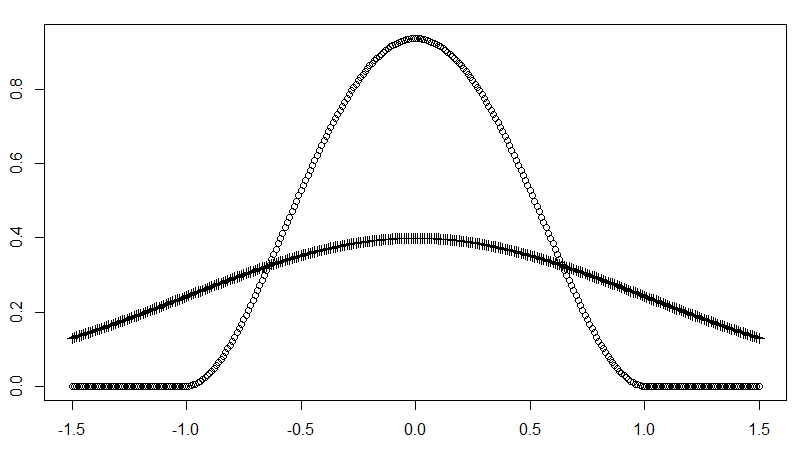
\includegraphics[width=5in]{1.png}

(f). 

By the formula in (b), we have
$$
I(\theta) =\int_{-1}^1 \frac{(\frac{15}{16} *2(1-x^2)*(-2x))^2}{\frac{15}{16} (1-x^2)^2} dx = 10
$$
in $\mathcal{F}$.

Form (d) and the property of the Normal distribution (Fisher information equals inverted variance), the Fisher information equals $7$ in $\mathcal{F}_N$.

(g).

As we can see, the C-R bound of $\mathcal{F}_N$ is higher which is easy to reach, since it has less Fisher information.

(h).

$\E(\bar{X}) = \E(\sum_i X_i / n) = \sum_i \E (X_i) /n = n\theta / n = \theta$. This shows that the sample mean is always an unbiased estimator for $\theta$.

(i).

The thing is that the two estimators has the same variance since $\var{\bar{X}} = \sigma_0/n$. This means that the two estimators has the same loss measure, indicating that they are of same efficiency.

(j). 

It is actually not. If you use the latter result which shows that the order statistic is the minimal sufficient statistic to improve the sample mean, it does not really help since the conditional expectation is still the sample mean.

In fact, most likelihood estimator will reach the C-R bound asymptotically. (Check MLE in the book or Internet.) Therefore it may be a good unbiased estimator. In all, you can see there are gaps between C-R bound and the variance of the sample mean, so it may have the space of improvement.

Pay attention that you may make mistakes by wildly conclude that it is UMVUE of some reason. It is not a easy job to say so.

(k). 

The density of the data is point mass $1/n!$ at the points which is a permutation of $(X_{(1)}, \ldots, X_{(n)})$. So it is free of $\theta$ which shows sufficiency.

(l).

Suppose the family is an exponential family. Then by the structure, $(\sum_i T_1(X_i) , \ldots, \sum_i T_s (X_i)$ is a sufficient statistic. Let $n > s$, then mapping $(X_{(1)}, \ldots, X_{(n)} )\rightarrow \sum_i T_1(X_i) , \ldots, \sum_i T_s (X_i)$ cannot be a bijection by simply checking the dimensions of the domain and the range. This contradicts with the fact that order statistic is minimal sufficient.

(m)

No. The sample mean is an unbiased estimator of $\theta$, and it is based on the order statistics. Note that $(X_{(1)} + X_{(n)})/2$ is also an unbiased estimator of $\theta$ by symmetry. Therefore define $\delta$ as the difference of the two estimators, and we have $\E_\theta(\delta) =0 $ while $\delta \neq 0$.

You can also use the fact that $X_{(n)} - X_{(1)}$ is an ancillary statistic in location family to show the incompleteness. (Check ancillary statistic if interested.)

(n)

The bias is always upwards since by Jensen's inequality:
$$
\E(e^X) \geq e^{\E X} = e^\theta.
$$
And since $\var{X} >0$, the inequality is strict.

% --------------------------------------------------------------
% You don't have to mess with anything below this line.
% --------------------------------------------------------------
\end{document} 